%% bare_adv.tex
%% V1.4
%% 2012/12/27
%% by Michael Shell
%% See: 
%% http://www.michaelshell.org/
%% for current contact information.
%%
%%*************************************************************************
%% Legal Notice:
%% This code is offered as-is without any warranty either expressed or
%% implied; without even the implied warranty of MERCHANTABILITY or
%% FITNESS FOR A PARTICULAR PURPOSE! 
%% User assumes all risk.
%% In no event shall IEEE or any contributor to this code be liable for
%% any damages or losses, including, but not limited to, incidental,
%% consequential, or any other damages, resulting from the use or misuse
%% of any information contained here.
%%
%% All comments are the opinions of their respective authors and are not
%% necessarily endorsed by the IEEE.
%%
%% This work is distributed under the LaTeX Project Public License (LPPL)
%% ( http://www.latex-project.org/ ) version 1.3, and may be freely used,
%% distributed and modified. A copy of the LPPL, version 1.3, is included
%% in the base LaTeX documentation of all distributions of LaTeX released
%% 2003/12/01 or later.
%% Retain all contribution notices and credits.
%% ** Modified files should be clearly indicated as such, including  **
%% ** renaming them and changing author support contact information. **
%%
%% File list of work: IEEEtran.cls, IEEEtran_HOWTO.pdf, bare_adv.tex,
%%                    bare_conf.tex, bare_jrnl.tex, bare_jrnl_compsoc.tex,
%%                    bare_jrnl_transmag.tex
%%*************************************************************************


\documentclass[12pt,journal,compsoc]{IEEEtran}

\usepackage[utf8]{inputenc}
\usepackage{listings}
\usepackage{hyperref}
\usepackage{graphicx}
\usepackage{float}
\usepackage{enumitem}
\usepackage[svgnames]{xcolor}
\usepackage{color}

\definecolor{pblue}{rgb}{0.13,0.13,1}
\definecolor{pgreen}{rgb}{0,0.5,0}
\definecolor{pred}{rgb}{0.9,0,0}
\definecolor{pgrey}{rgb}{0.46,0.45,0.48}
\hypersetup{
  colorlinks=false,
  linkbordercolor={white}
}

\lstset{language=Java,
  showspaces=false,
  showtabs=false,
  breaklines=true,
  showstringspaces=false,
  breakatwhitespace=true,
  commentstyle=\color{pgreen},
  keywordstyle=\color{pblue},
  stringstyle=\color{pred},
  basicstyle=\ttfamily,
}


\newcommand\MYhyperrefoptions{bookmarks=true,bookmarksnumbered=true,
pdfpagemode={UseOutlines},plainpages=false,pdfpagelabels=true,
colorlinks=true,linkcolor={black},citecolor={black},urlcolor={black},
pdftitle={Práctica 3},
pdfsubject={Programación Distribuida y Tiempo Real - Práctica 2},
pdfauthor={Lucas Di Cunzolo,Santiago Tettamanti},
pdfkeywords={Programación Distribuida y Tiempo Real, java, LaTeX, rmi}}

\hyphenation{op-tical net-works semi-conduc-tor}

\begin{document}
\title{Práctica 3\\Programación Distribuida y Tiempo Real}
\author{Lucas Di Cunzolo\\Santiago Tettamanti}

\IEEEtitleabstractindextext{%
\begin{abstract}
Remote Method Invocation
\end{abstract}

\begin{IEEEkeywords}
Programación Distribuida y Tiempo Real, java, \LaTeX, RMI
\end{IEEEkeywords}}

\maketitle

\IEEEdisplaynontitleabstractindextext
\IEEEpeerreviewmaketitle

\section{Punto 1}

\textit{Utilizando como base el programa ejemplo de RMI}
\begin{enumerate}[label=\alph* -]
  \item \textit{Analice si RMI es de acceso completamente
  transparente (access transparency, tal como está definido en
  Coulouris-Dollimore-Kindberg). Justifique}

  Colouris:
     Access transparency. Enables local and remote resources to be
     accessed using identical operations They both offer a similar level
     of transparency that is, local and remote calls employ the same
     syntax but remote interfaces typically expose the distributed nature
     of the underlying call, for example by supporting remote exceptions

  Vemos que sintácticamente las operaciones son idénticas y no se podría
  saber si la operación es local o remota dado que el los nombres de las
  operaciones son exactamente los mismos. sin embargo a la hora de llamar
  a la clase hay que hacer un lookup del nombre de esta, al no estar en
  el espacio de nombres local, teniendo el cuenta el hostname remoto.
  Por lo que si bien a nivel invocación de métodos nunca no enteramos si
  es local o remoto y no se hace ninguna diferencia en la invocación de
  ambos, a la hora de obtener la clase remota si. Todo esto sin tener en
  cuenta el manejo de posibles errores en la comunicación ya que el método
  remoto tiende a fallar mucho más seguido que el local mayormente por fallas
  en la comunicación que son inexistentes en el otro.
  En conclusión, teniendo en cuenta lo definido en el libro, RMI si ofrece
  una tranparencia de acceso al permitir invocar tanto un procedimiento
  local como remoto de la misma manera. Pero esa transparencia no es total
  ya que hay que tener en cuenta otras cuestiones como el lookup de la clase
  remota y la posible falla en la comunicación.\\

  \item \textit{Enumere los archivos .class que deberían estar del lado
  del cliente y del lado del servidor y que contiene cada uno.}

  \begin{itemize}
    \item \textbf{AskRemote.class:} Presente en el cliente, identifica a
    la clase cliente que realiza el llamado al metodo remoto. Contiene,
    entre otras cosas, información de conexión al servidor tal como su
    hostname, invocación a la clase y al método remoto.\\

    \item \textbf{StartRemoteObject.class:} Presente en el servidor.
    Es la clase encargada de instanciar a la clase contenedora de los
    métodos remotos a invocar y la registra en el espacio de nombres
    asegurándose que pueda ser llamada por el cliente.\\

    \item \textbf{IfaceRemoteClass.class:} Presente en el servidor;
    es la interface que define los métodos que pueden ser invocados y
    que la clase del servidor debe implementar.\\

    \item \textbf{RemoteClass.class:} Presente en el servidor;
    solo implementa los métodos que serán invocados remotamente
    presentes en la interfáz mencionada anteriormente. Extiende de
    UnicastRemoteObject, lo que hace toda la comunicación totalmente
    transparente al programador desde este lado.\\
  \end{itemize}
\end{enumerate}

\section{Punto 2}
\textit{Identifique similitudes y diferencias entre RPC y RMI.}

La principal diferencia entre RPC y RMI es que RMI involucra objetos.
En lugar de llamar procedimientos de forma remota llama a métodos de
objetos remotos. Se podría decir que RMI es la version orientada a objetos
de RPC.  En RMI cada objeto tiene una referencia única en todo el sistema,
tanto si los objetos son remotos como locales, permitiendo así el pasó de
objetos como parámetros, herencia y relaciones entre objetos remotos,
ofreciendo un pasaje de parámetros con una mayor riqueza semántica y un
mayor nivel de abstracción que en RPC, donde solo se pueden pasar
parámetros por valor.

En ambos modelos los detalles de implementación están ocultos al usuario
y los métodos o procesos disponibles se conocen a través de una interfaz
que provee el servidor.
Ambos ofrecen un alto nivel de transparencia de acceso, llamadas remotas
y locales poseen la misma sintáxis pero las interfaces remotas
diferencian la naturaleza distribuida de las llamadas remotas al, por
ejemplo, soportar excepciones remotas o tener en cuenta posibles fallas
en la comunicación con tiempos de timeout.

\section{Punto 3}

\textit{Investigue porque con RMI puede generarse el problema de
desconocimiento de clases en las JVM e investigue como se resuelve este
problema.}\\

En rmi puede ser que los métodos de un objeto remoto admitan como parámetros a otras clases y devuelvan clases.  Por lo que un metodo remoto podría devolver un objeto o admitir un parámetro de una clase desconocida para el cliente. En ese caso se podría generar una ClassNotFoundException
Por ejemplo, puede ser un método así

public InterfaceResultado dameResultado (InterfaceParametro parametro) throws java.rmi.RemoteException
{
   ...
}


Una solucion sería que  tanto el servidor como el cliente tengan sus propias copias de las clases que implementen estas interfaces. Es decir, si ClaseResultado implementa InterfaceResultado y ClaseParametro implementa InterfaceParametro, tanto el cliente como el servidor deben tener en su CLASSPATH los ficheros ClaseResultado.class y ClaseParametro.class. Esto no sería una solucion deseada, ya que se deben saber todas las clases que utiliza el servidor y copiarlas del lado del cliente, quitando dinamismo y escalabilidad a rmi.
 La solución provista por RMI es instalar RMISecurityManager, el cual habilita la carga dinámica de clases. De esta forma el servidor no necesita tener una copia de ClaseParametro.class ni el cliente una copia de ClaseResultado.class. 


\section{Punto 4}

\textit{Implementar con RMI el mismo sistema de archivos remoto
implementado con RPC en la práctica anterior:}

\begin{enumerate}[label=\alph* -]
  \item \textit{Defina e implemente con RMI un servidor y un cliente con
  un copiado de archivos con backup}\\\\
  
  Para esto se utilizó la estructura de archivos del ejemplo. Se definió
  una interfaz con 3 métodos, \textit{read}, \textit{write} y
  \textit{list}
  Tanto el cliente como el servidor, se alimentan de la interfaz definida
  en la clase IfaceRemoteClass.
  \hyperref[section:IfaceRemoteClass]{(Ver apéndice - Subsección IfaceRemoteClass)}
  
  Donde la clase que los implementa es la RemoteClass
  \hyperref[section:RemoteClass]{(Ver apéndice - Subsección RemoteClass)}\\
  
  Luego se implementó un cliente que interactúe contra el servidor, con
  los comandos basicos, nombrados anteriormente. Esto se hizo en la clase
  AskRemote
  \hyperref[section:AskRemote]{(Ver apéndice - Subsección AskRemote)}

  El servidor, utiliza la implementación de la clase RemoteClass, y
  corre instanciando un objeto de la clase StartRemoteObject.
  \hyperref[section:StartRemoteObject]{(Ver apéndice - Subsección StartRemoteObject)}

\end{enumerate}

\section{Punto 5}

Investigue si es posible que varias invocaciones remotas estén
ejecutándose concurrentemente y si esto es apropiado o no para el
servidor de archivos del ejercicio anterior. En caso de que no sea 
apropiado, analice si es posible proveer una solución
(enunciar/describir una solución, no es necesario implementarla).

Nota: diseñar un experimento con el que se pueda demostrar
fehacientemente que dos o más invocaciones remotas se ejecutan
concurrentemente o no. Compare este comportamiento con lo que sucede con
RPC.\\\\
Al funcionar sobre Java, RMI admite concurrencia nativa.
El principal inconveniente en RMI, es que no maneja multihilos de manera
segura, es decir, los llamados pueden causar colisiones en los recursos
del servidor.\\
Para evitar esto, se pueden utilizar mecanismos conocidos para sincronización,
aunque RMI no provee ninguno por su cuenta.\\
En nuestro caso, contamos con 2 comandos seguros para la concurrencia, estamos
hablando de los comandos \textit{read} y \textit{list}, mientras que contamos con
comandos como \textit{write} y \textit{readwrite} los cuales no lo son.\\
El principal inconveniente que puede traer la ejecución de comandos no seguros, es
la perdida de datos en el servidor.\\
Para mayor información de manejo de hilos con RMI, se consultaron foros.\\
\hyperref[section:links]{Ver apéndice - Subsección Links}

Para demostrar la concurrencia de RMI, se utilizó un comando extra, para
mayor simplicidad del experimento.\\
En este caso, el método remoto solamente genera un sleep de 6 minutos.\\
\hyperref[fig:concurrecia]{Ver captura}\\
En la captura se puede observar como ambos clientes ejecutan concurrentemente
el comando \textit{timeout} sin ningún problema.

\section{Punto 6}

Tiempos de respuesta de una invocación:

\begin{enumerate}[label=\alph* -]
  \item Diseñe experimento que muestre el tiempo de respuesta mínimo de
  una invocacióncon JAVA RMI. Muestre promedio y desviaciónestándarde
  tiempo respuesta.

  Se ejecutó 500 veces un comando, y se guardo el tiempo de respuesta,
  con eso se calculó la media y la desviación estándar.\\

  \hyperref[section:times]{(Ver apéndice - Subsección Tiempos de ejecución)} \\

  Se puede volver a generar el archvio corriendo el script \textit{get\_data}
  el cual acepta como primer parametro la cantidad de iteraciones y como
  segundo parámetro el nombre de archivo donde dejar los valores.\\

  \item Investigue los timeouts relacionados con RMI. Como mínimo,
  verifique si existe un timeout predefinido. Si existe, indique de
  cuantoes el tiempo y si podría cambiarlo. Si no existe, proponga alguna
  forma de evitar que el cliente quede esperando indefinidamente.\\

  El paquete \textbf{java.rmi} no cuenta con timeout configurable,
  se puede utilizar el paquete \textbf{sun.rmi}, el cual cuenta con una
  propiedad configurable de timeout.

  De no utilizarse \textbf{sun.rmi}, se pueden llegar a trabajar con algun
  timer o algo similar, pero no hay ninguna herramienta que nos brinde 
  \textbf{java.rmi} para dicho fin.

\end{enumerate}

\newpage
\onecolumn
\appendix{Código Java}
\label{appendix:codigo-java}

\subsection{IfaceRemoteClass}
\label{section:IfaceRemoteClass}
\lstinputlisting[language=Java, firstline=7    ]{../IfaceRemoteClass.java}

\subsection{AskRemote}
\label{section:AskRemote}
\lstinputlisting[language=Java, firstline=6]{../AskRemote.java}

\subsection{RemoteClass}
\label{section:RemoteClass}
\lstinputlisting[language=Java, firstline=8]{../RemoteClass.java}

\subsection{StartRemoteObject}
\label{section:StartRemoteObject}
\lstinputlisting[language=Java, firstline=7]{../StartRemoteObject.java}

\subsection{Tiempos de ejecución}
Ver archivo completo en \textbf{code/times}\\
Los valores se encuentran en \textbf{nanosegundos}
\label{section:times}
\lstinputlisting[firstline=495]{code/times}

\subsection{Links}
\label{section:links}
Documentación de propiedades del paquete \textbf{java.rmi}\\
https://docs.oracle.com/javase/8/docs/technotes/guides/rmi/javarmiproperties.html\\\\
Artículos de multithread
\begin{itemize}
  \item Java RMI and Thread Synchronization questions\\\url{https://stackoverflow.com/questions/2275868/java-rmi-and-thread-synchronization-questions}
  \item Java RMI and synchronized methods\\\url{https://stackoverflow.com/questions/3507253/java-rmi-and-synchronized-methods/3629723}
\end{itemize}

\subsection{Capturas}
\label{section:capturas}
\begin{figure}[H]
  \centering
  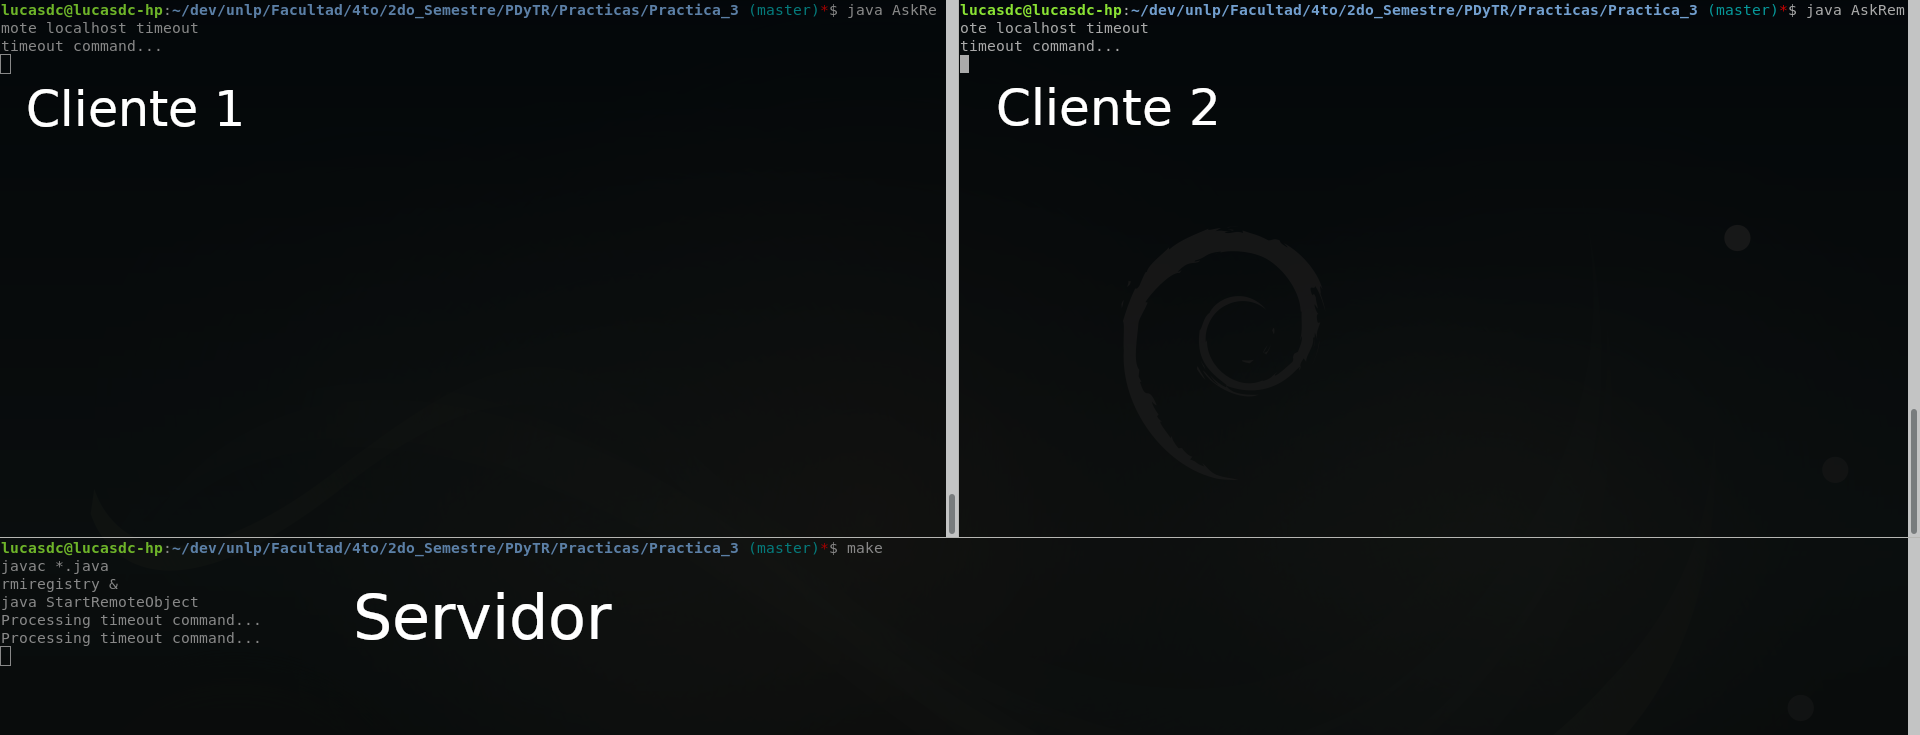
\includegraphics[width=180mm]{capturas/concurrencia.png}
  \caption{Experimento concurrecia}
  \label{fig:concurrecia}
\end{figure}

\ifCLASSOPTIONcaptionsoff
  \newpage
\fi
\end{document}
